\chapter{方法框架与设计}
在本章中,我们提出并详细描述我们在 \cu 的基础上构建的单元格聚类和缺陷检测技术\wa 。
我们首先介绍 \wa 的方法框架,以及它和 \cu 的结构关系。
之后,我们详细介绍 \wa 的三个基于有效性属性的单元格聚类检验方法。


\section{框架描述}
如图\ref{figure1}所示,\wa 和 \cu 集成在一起,包含 4 个阶段:两阶段的单元格聚类、单元格类检验和公式缺陷检测。

首先,\wa 使用 \cu 的第一阶段来生成一个包含若干个种子单元格类的集合,每个种子类中的任意一个单元格都包含明显相似的计算特征,即\textit{强特征}(例如公式表达式的语法树结构,以及公式表达式的单元格引用结构)。
这个阶段使得每个种子类都包含一个高度相似的计算语义。

第二,\wa 使用 \cu 来扩充每个种子类,将还没被吸纳进任何类中的数值单元格和公式单元格作为对象,只要这些单元格和在第一阶段已经在种子类中的单元格拥有相似的单元格布局或潜在的计算特征,即\textit{弱特征}(例如单元格位置、单元格表头信息、以及是否隶属于相同的单元格模板等)。
这个阶段是将在第一阶段被忽视的单元格重新吸纳起来,这些被忽视的单元格通常由于自身含有某种公式缺陷,因而在第一阶段中被忽略。

第三,\wa 检验第二阶段得到的单元格类,通过将那些违反有效性属性的单元格(后面三节会详述这三种有效性属性)从它所属的类中排除,或者将整个违反有效性规则的单元格类直接移除。
这个阶段通过识别与对应类的计算语义不相关的单元格和不合格的单元格类,来提升单元格聚类的准确性。

第四,\wa 使用 \cu 从每个单元格类中识别出含有公式缺陷的单元格,并把这些单元格汇报给终端用户。
这个阶段是在含有共同计算语义的单元格类中检测第三章定义的三类公式缺陷,即用数值替换的公式缺陷、用单元格引用替换的公式缺陷和用操作符/函数替换的公式缺陷。

\cu 的优点在于能够将许多零散分布的单元格吸纳到种子类中,从而提升了单元格聚类和缺陷检测的召回率\cite{cheung2016custodes}。
然而,这一吸纳过程比较激进,因为它同时也将相当数量的与单元格类的计算语义不相关的单元格吸纳进来,影响了单元格聚类和缺陷检测的精度。
正因如此,这一不足之处正是我们的技术 \wa 提出的三个检验方法想要解决的痛点,接下来我们详细描述检验单元格和单元格类的方法细节。
\begin{figure}[tbp]    
    \centering
    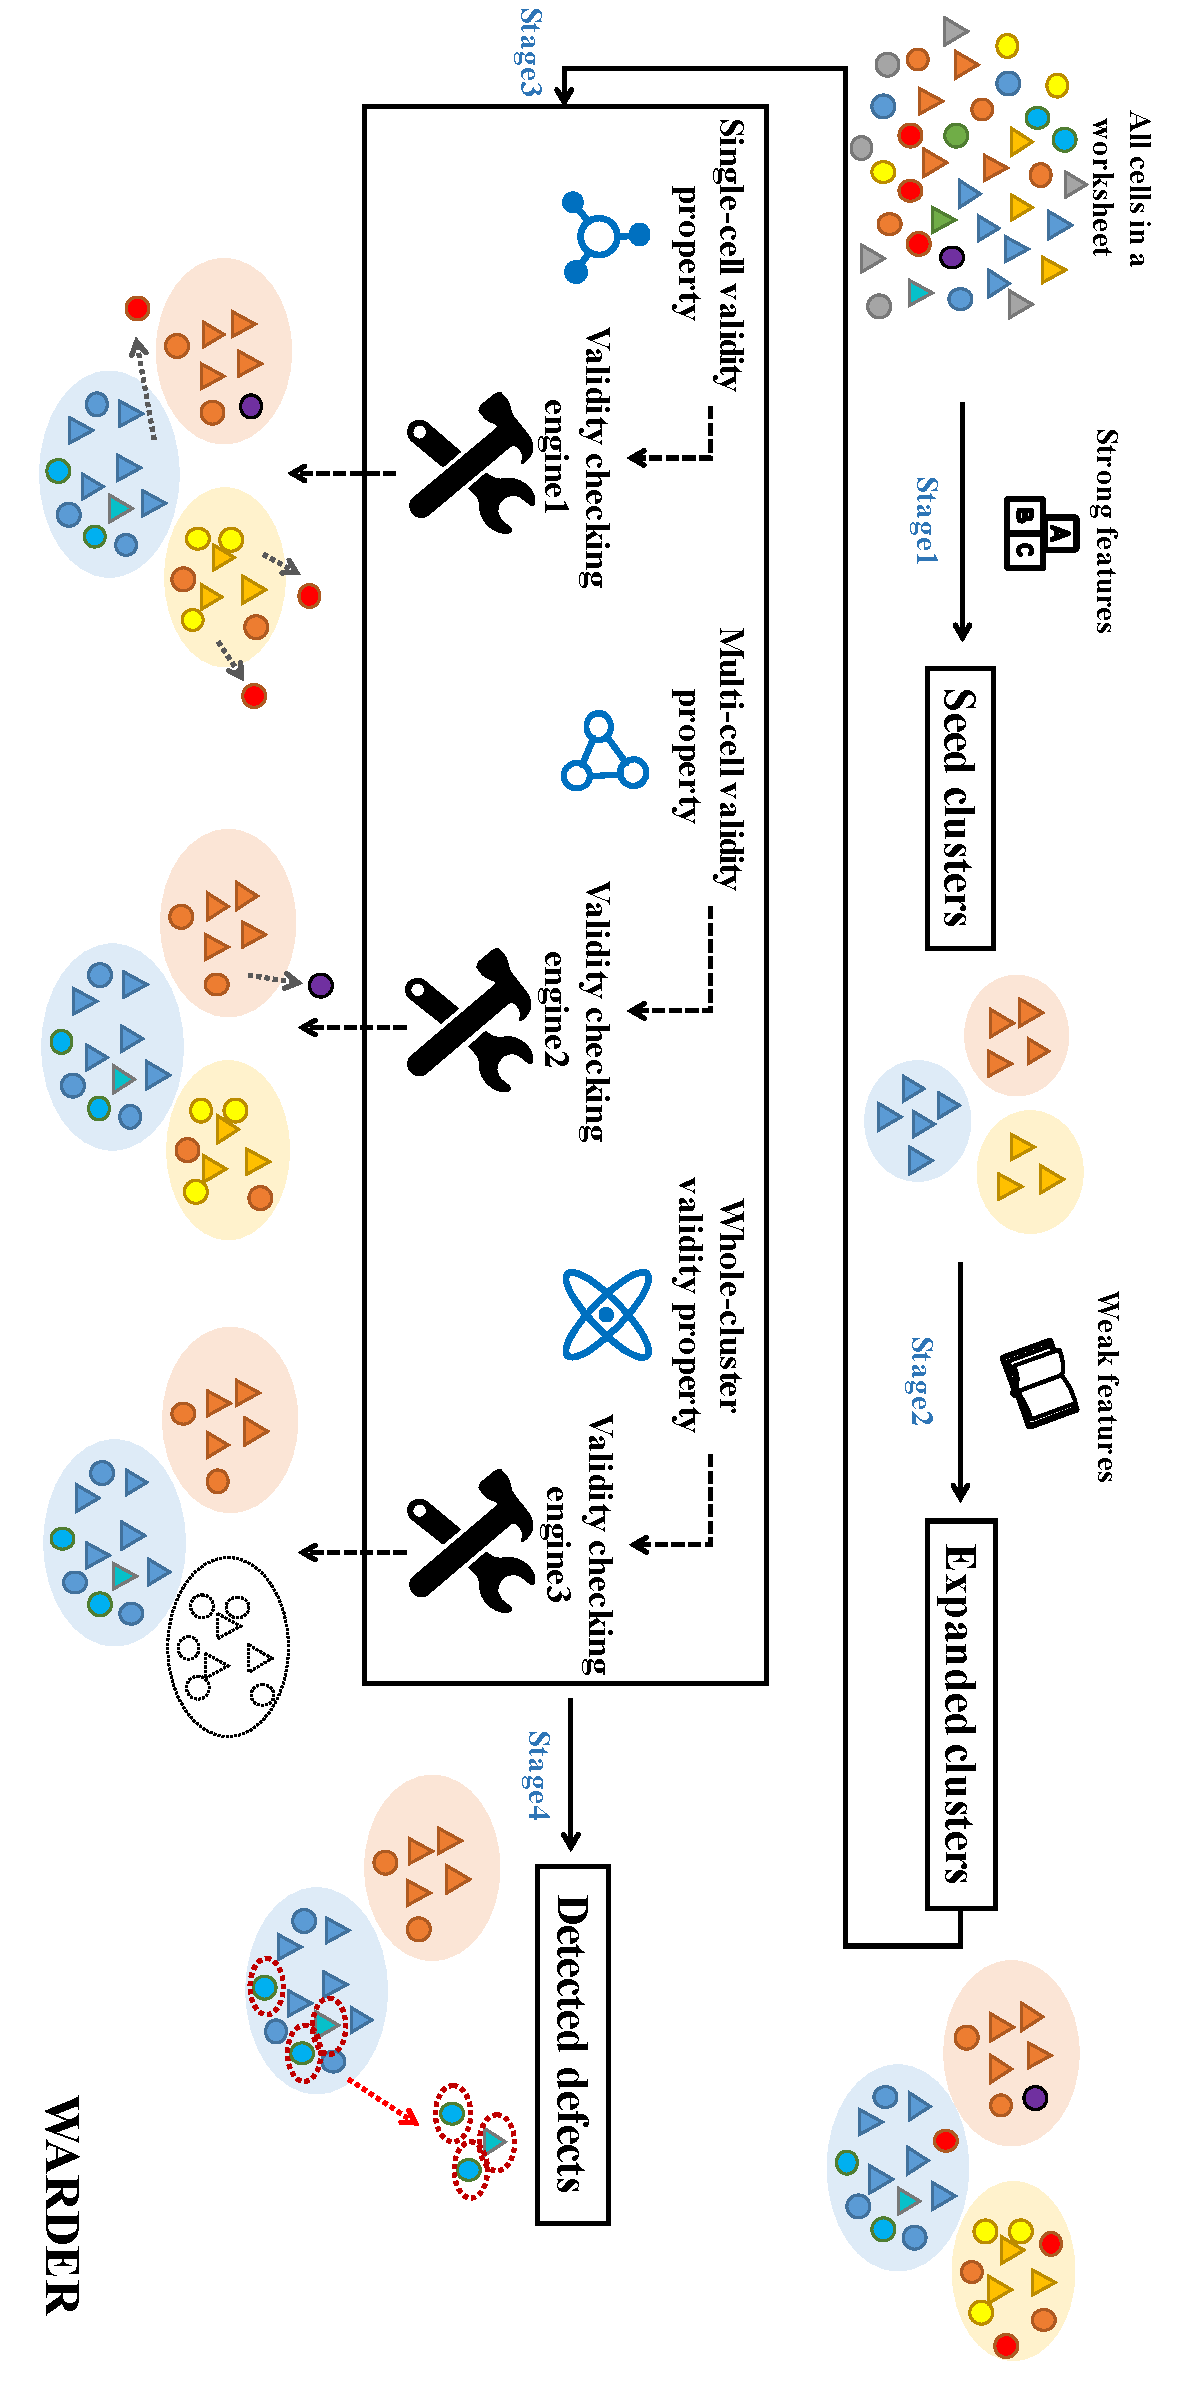
\includegraphics[width=0.7\textwidth]{figure/figure1-copy.pdf}
    \caption{\wa 的工作流程(阶段 3 是相对于它的前身 \cu 的核心贡献点)}
    \label{figure1}
\end{figure}


\section{针对单元格自身的有效性检验}
\begin{figure}[tbp]
    \centering
    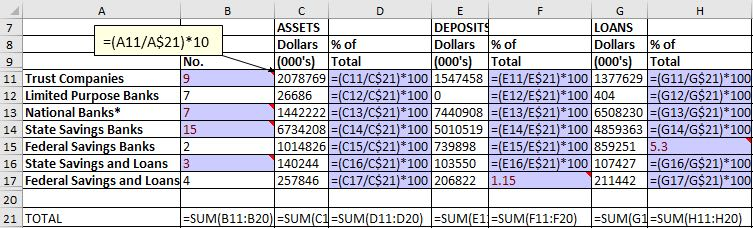
\includegraphics[width=\columnwidth]{figure/figure2.png}
    \caption{用于展现\wa 的单个单元格有效性精化方法的工作表``Summary1201''。\cu 检测出一个单元格类(用紫色标记),导致四个误报的缺陷(用红色三角标注),不过这四个单元格会被\wa 的单个单元格有效性精化方法排除出去,也就不再被错误标记为缺陷。}
    \label{figure2}
\end{figure}
第一个有效性检验方法考虑的是,当 \wa 准备将数值单元格扩充到种子类中的时候,这些被扩充的数值单元格自身是否可能拥有和种子类的计算语义相似的可能性。

在实际情况下,并没有直接的 方法可以判断这些数值单元格的有效性,换言之,因为它们仅包含纯数值,无法从它自身找出和其它单元格之间的任何明显的计算语义关系。
不过,因为这些被扩充的单元格和种子类中的公式单元格即将被纳入同类,那么根据第三章中对单元格类的定义,它们应该享有一个相似的计算目标。
那么,这些被扩充的单元格的数值应当可以用某个公式单元格中含有的表达式计算出来,这是一种对数值单元格较强的约束。

为了验证这一约束,\wa 会枚举种子类中所有单元格的公式,“复制并粘贴”该公式到数值单元格中,来判断是否至少存在一个公式的计算结果和被扩充的这个单元格的值保持一致,如果保持一致,则称该数值单元格满足\textit{强有效性属性}。
但同时又考虑到如果数值单元格本身是含有缺陷的,那复制的公式计算的结果可能和原来的数值不同。因此,我们放宽了约束条件,当我们用一个公式来替换当前数值单元格里的内容时,只要该单元格是可计算的,即称为满足\textit{弱有效性属性}。
相反地,如果所有复制的公式都是不可计算的,例如复制的公式引用了错误的单元格类型,或本身包含了无效的单元格引用(比如越界),这个被扩充的数值单元格就是不满足弱有效性的,会被阻止扩充进该类中。
我们把这种方法就称为\textit{针对单元格自身的有效性检验}。
% 这里可以解释一下什么是 “用公式替换数值” 的思路

接下来,我们形式化地描述一下该检验方法。在前两个阶段得到的某一个种子类记为$SC$,对应的拓展类记为$EC$。
种子类本身是个集合,包含若干个公式单元格,记为$SC= \{c_{1}, c_{2}, \dots, c_{n}\}$,种子类中的所有公式合集记为$F_{SC}$。
同理,对应的拓展类也包含多个公式单元格,记为$EC=\{c_1, c_2, \dots, c_n, \dots, c_m\}$,其中$n \leq m$,拓展类中的所有公式合集记为$F_{EC}$。
用$eval(f|_c)$表示在单元格$c$的位置用公式$f$计算得到的数值。
当前等待检验的数值单元格记为$c_v$,它存储的数值为$v$。
上述提到的公式统一用 R1C1 表示法,原因正如第三章所述。

那么上述自然语言描述的强有效性属性定义如下:
\begin{definition}
    如果 $\exists f \in F_{SC},  eval(f|_{c_v}) = v$,那么就称数值单元格$c_v$满足被吸纳进$SC$中的强有效性属性。   
\end{definition}

对应地,弱有效性属性定义如下:
\begin{definition}
    如果 $\exists f \in F_{SC}, eval(f|_{c_v})$的计算过程不会触发异常,即是可计算的,那么就称数值单元格$c_v$满足被吸纳进$SC$中的弱有效性属性。
\end{definition}

这里我们要额外解释一下$f|_{c_v}$的含义。
该过程指用$F_{SC}$中的某个公式$f$复制粘贴到单元格$c_v$中,结合第三章对公式表达式的定义,复制粘贴过程中常量、操作符、函数名、单元格引用都保持不变。
我们在实际 \wa 的实现中,使用弱有效性定义来检验单元格自身。
因为即便不能在聚类时直接确认该数值单元格具有公式缺陷,在后续的缺陷检测过程中,数值单元格仍旧会被标注为含有用常量替换的公式缺陷,并不影响最终的检测结果。

\subsection*{案例分析}
如图\ref{figure2}所示,工作表“Summary1201”给出了一个案例,其中 25 个单元格(B11,B13,B14,B16,D11-17,F11-17和 H11-17)被\cu 划分为同类(用紫色标注)。
\cu 检测出了 6 个缺陷(用红色三角标注),其中 2 个(F17 和 H15)是真阳性,另外四个(B11,B13,B14 和 B16)是假阳性。
后四个数值单元格被扩充进这个类,是因为它们具有和种子类中单元格类似的弱特征(例如相似的表头和布局)。

然而,根据 \wa 的单个单元格有效性检验方法,这样的扩充是有问题的。
事实上,如果这四个单元格中的任意一个被扩充到这个类中,这个单元格把它的值和任意一个类中包含的公式计算出来的值相一致。
例如,考虑单元格 B11,按照类中包含的公式来看,对于它来说最好的潜在公式应该是“=(A11$/$A\$21)$*$100”。
然而,这个公式是不可计算的,因为单元格 A11 和 A\$21指向字符串单元格,无法参与这类除法算数运算中。
相似的问题也出现在单元格 B13、B14 和 B16。 
因此,\wa 会阻止这类数值单元格被扩充到类中。


\section{针对单元格之间关系的有效性检验}
第二个有效性检验方法考虑的是,当 \wa 用额外的数值单元格扩充种子类时,这类被扩充进来的单元格不会破坏种子类中已有单元格之间的属性。

我们拿单元格的引用举例,因为这是电子表格单元格的重要特征。
假设种子类中已有单元格的引用从不会彼此重叠,那么我们会预期一个被扩充进来的数值单元格当它被加入到这个类中,并且它的值被类中某个其他单元格的公式替换时,也不会违反这个属性。
这个预期也可以用一种相反的方式表达出来,即一个单元格类中的已有公式之间的引用已经彼此重叠了,那么对于被新扩充进来的数值单元格也不能发生不相交的情况。
也就是说,这个属性应当对类中所有的单元格保持一致(不管是原有的单元格,还是被扩充进来的单元格),这可以被看作电子表格中标的编辑风格。
另外,如果检测到违反该一致性的数值单元格,它就应当被禁止扩充到这个类中。
我们把这种方法称为\textit{针对单元格之间关系的有效性检验}。

接下来,我们形式化地描述一下该检验方法。
对引用集合交集均为空集的定义如下:
\begin{definition}
    假如$\forall c_i,c_j \in SC,\psi(f_i|_{c_i}) \cap \psi(f_j|_{c_j}) = \emptyset$,其中$f_i$为$c_i$的公式,$f_j$为$c_j$的公式,
    那么对于数值单元格$c_v$而言,如果$\exists f_k \in F_{SC}, \forall c_i \in SC, \psi(f_k|_{c_v}) \cap \psi(f_i|_{c_i}) = \emptyset$,
    则称单元格$c_v$满足针对单元格之间关系的空集有效性属性。
\end{definition}

相应地,对引用集合交集均为非空的定义如下:
\begin{definition}
    假如$\forall c_i,c_j \in SC,\psi(f_i|_{c_i}) \cap \psi(f_j|_{c_j}) \neq \emptyset$,其中$f_i$为$c_i$的公式,$f_j$为$c_j$的公式,
    那么对于数值单元格$c_v$而言,如果$\exists f_k \in F_{SC}, \forall c_i \in SC, \psi(f_k|_{c_v}) \cap \psi(f_i|_{c_i}) \neq \emptyset$,
    则称单元格$c_v$满足针对单元格之间关系的非空集有效性属性。 
\end{definition}

在第三章我们定义过针对公式表达式的引用集合$\sigma(exp)$,这里的$\psi(f|_c)$类似,表示将 R1C1 表示法下的公式$f$套用在单元格$c$上,单元格$c$实际引用的具体单元格集合。比如单元格C3套用上公式RC[-2]+RC[-1],则对应的$\sigma$(RC[-2]+RC[-1])为\{RC[-2],RC[-1]\},而$\psi$((RC[-2]+RC[-1])$|_{C3}$)为\{A3,B3\}。

\subsection*{案例分析}
\begin{figure}[tbp]
    \centering
    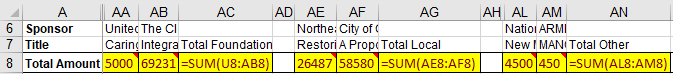
\includegraphics[width=\columnwidth]{figure/figure3.png}
    \caption{用于展现\wa 的多个单元格有效性精化方法的工作表``Detail for the College of A\&S''。\cu 检测出一个单元格类(用黄色标记),并进而导致六个假阳性的缺陷被报告出来(用红色三角形标注),不过这六个单元格会被\wa 的多单元格有效性精化方法从类中排除出去,进而不会再被错误的标记为有缺陷的单元格。}
    \label{figure3}
\end{figure}
如图\ref{figure3}所示,工作表“Detail for the College of A\&S” 给出了一个案例。
其中,9 个单元格(AA8, AB8, AC8, AE8, AF8, AG8, AL8, AM8和AN8)被\cu 划分到同一个类中(用黄色标记)。
接着,\cu 检测出 6 个单元格缺陷(AA8, AB8, AE8,AF8,AL8和AM8),因为它们只包含纯数值,但这六个缺陷都是假阳性。

不过,\wa 能够阻止这六个单元格(AA8, AB8, AE8,AF8,AL8和AM8)被扩充进来,从而避免了这 6 个误报的情况。
事实上,这 6 个数值单元格并不和其它 3 个公式单元格(AC8,AG8和AN8)共享相同的计算语义。
前面的数值单元格代表了用户直接给出的具体的数值,而另外三个公式则是计算它们各自左侧的若干个单元格的和。

\wa 通过它的多个单元格有效性检验方法区分出这两类:后三个公式单元格的引用范围是互不重叠的,但如果把前面 6 个数值单元格扩充进来,并用任意一个公式来替换它们的值,这个属性会遭到破坏。
例如,当把单元格 AF8 中的数值用单元格 AG8 里的公式模板替换成公式“=SUM(AD8:AE8)”时,它的引用单元格(AD8 和 AE8)会和单元格 AG8 的引用单元格(AE8 和 AF8)发生重叠。
相似的问题也会出现在单元格 AA8,AB8,AE8,AL8 和 AM8 上。
因此,\wa 会禁止这类数值单元格被扩充到类中。


\section{针对整个类的有效性检验}
第三种有效性检验方法考虑的是最终形成单元格类的整体有效性,即它关注于类层面而不是单元格层面的有效性属性。

我们预期在每个单元格类中应该存在一个统一的公式能够覆盖大多数单元格,也就是说大多数单元格应当遵循一个共同的计算语义。
\wa 会测试类中所有现存可获得的公式,如果没有任何一个能够满足这个目的,\wa 就会认定这个类不是有效的,并将该类从所有类的集合中删除,以避免后续在缺陷检测过程中将其中的过半数量的单元格标记为含有公式缺陷,即产生大量缺陷误报。
我们把这种方法称为\textit{针对整个类的有效性检验}。

接下来,我们形式化地描述一下该检验方法。
我们首先定义一个辅助函数:
\begin{definition}
    对于一个公式$f_i \in F_{EC}$和某个公式单元格$c$及其自身包含的公式$f$来说,定义辅助函数$\rho$为
    $
    \rho(f_i, c) = 
    \left\{
        \begin{aligned}
        & 1     & eval(f_i|_c) == eval(f|_c); \\
        & 0     & otherwise. \\
        \end{aligned}
    \right.
    $
    如果$\rho(f_i,c)$为 1,则我们称公式$f_i$可以用来覆盖单元格$c$且计算出的新值与原有公式计算的值相等。
\end{definition}

接着我们定义:
\begin{definition}
    如果$\exists f_i \in F_{EC}, (\sum_{j = 1}^{m} \rho(f_i, c_j)) > \theta  * size(F_{EC})$,
    则我们称该扩展单元格类存在一个能覆盖超过$\theta  * size(F_{EC})$数量的公式单元格的统一公式,即该单元格类满足针对整个类的强有效性属性。
\end{definition}

如果我们把辅助函数等于 $1$ 的条件适当放宽,即要求$\frac{|eval(f_i|_c)-eval(f|_c)|}{eval(f|_c)} \leq \epsilon$,即新值与旧值的差的绝对值占旧值的比例小于给定的阈值$\epsilon$,
则相应地,我们就得到了关于该单元格类满足针对整个类的弱有效性定义。在实验评估中,$\epsilon$取值为0.01,即我们容忍较小程度的计算结果偏差,如果偏差较大,说明该单元格很可能不应该被此公式覆盖。
我们这里只是枚举公式集合$F_{EC}$中的公式来尝试覆盖整个单元格类,而没有使用类似基于组件的程序合成方法来为整个类合成一个最为适宜的公式。
这样的做法有两点考虑:第一,使用程序合成算法通常会大大降低执行效率,让终端用户的等待时间更久;
第二,每个单元格类中的公式通常比较简单,相似度高,在公示集合中存在备选公式的概率较高,没有必要动用相对复杂的程序合成工具。

在\wa 的实际系统实现中,我们采用针对整个类的弱有效性定义来过滤不合格的单元格类,因为我们要容忍某些公式单元格是有缺陷的,因而计算出来的值有一定偏差可以允许。
在后续的缺陷检测环节,我们有很大把握将其检测出来。

\subsection*{案例分析}
\begin{figure}[tp]
    \centering
    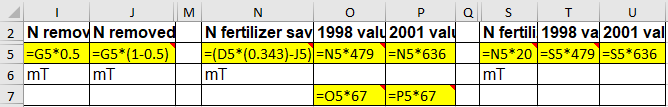
\includegraphics[width=\columnwidth]{figure/figure4.png}
    \caption{用于展现\wa 的整个类有效性检验方法的工作表``World 1996''。\cu 识别出了一个类(用花色标记出来,但整个类是不合理的),进而导致所有相关的单元格都被错误地标记为有缺陷的(用红色三角形标记),不过这个类会被\wa 的整个类的有效性检验方法移除掉,进而相关的所有单元格也不会被错误地标记为有缺陷的。}
    \label{figure4}
\end{figure}
如图\ref{figure4}所示,工作表“World 1996”给出了一个案例。
其中,\cu 把 10 个单元格划分为同一个类(用黄色标注)。
进而 \cu 把其中的 7 个检测为有缺陷的单元格,但这 7 个都是假阳性。

事实上,这10 个单元格包含几乎完全不同的公式(5 种计算模式),这强烈地表明它们本质上遵循不同的计算语义。
通过我们的类级别的有效性检验方法,\wa 会将该类完整地从类集合中删除。
这里需要注意的是,\wa 需要一个阈值来控制“覆盖大多数单元格”这个判断的程度,即确定阈值$\theta$。
安全起见,\wa 选择一个保守的值,即 50\%,来尽可能保护单元格类不被排除在外(作为对比,\ca 选择了相对激进的值70\%)。


\section{有效性检验的综合应用}
其实前面三节我们给出了设计有效性检验方法的逻辑框架,本文仅是在三个层面上分别设计了最为基础但也最为实用的有效性检验方法,在第六章的实验评估中也取得了较好的效果,说明进行有效性检验方法本身的思路是成立的,的确解决了\cu 存在的技术缺陷,未来工作可以在三个层面上进行更细致的有效性检验方法设计和改良。

根据上述设计的三个有效性检验方法之间的层次关系,\wa 将三个方法依次应用在 \cu 的第二阶段单元格聚类之后,即依次使用针对单元格自身、针对单元格之间关系和针对整个类的有效性检验方法。
它们三者彼此互补,构成了针对单元格聚类的有效性检验方法的有机整体。
它们的目标是提升单元格聚类有效性,使得聚类结果更加具有稳定和可靠。

稳定可靠的单元格聚类结果,最终也会对缺陷检测起到积极作用,如极大地减少公式缺陷的误报数量和误报率,这部分也会在第六章的实验评估部分进行验证。